\section{3 related work}
\subsection{Stationary and true mobile spatial navigation in VR}
Modern virtual reality headsets provide precise motion capture and conversely allow to render a wide variety of motion illusions useful for research in spatial navigation. Using lightweight electrical (Electroencephalogram, EEG) or optical (functional near infrared spectroscopy, fNIRS) sensors concurrently, it is now feasible to digitize brain signals along with spatial location. However, different systems impose different requirements on the participants. Those technical requirements may in turn affect participants experiences, such as feeling present, in VR. \cite{} % todo effect of wires on presence
We consider a minimum of three different levels of continuous self-motion perception in head-mounted VR in the evolution from constrained stationary to unconstrained freely movements. On the first level we locate perceiving illusory motion, i.e. vection, induced through flow signals. Such flow signals can be sensible by a number of different senses, e.g. optical flow by the visual sense or wind flowing over the skin. Vection can be induced in completely immobile participants and is hence compatible with a great number of brain imaging technology that require participants to remain stationary, i.e. fMRI and MEG. The strength of the vection illusion can be significantly increased by minimal physical motion cueing \cite{}. %Riecke/Cruiff motion cueing \cite{} %Riecke arbeiten
Such physical motion cues briefly trigger the vestibular and proprioceptive sensing systems in addition to the senses perceiving flow signals. Interestingly, such cues can be delivered without physically moving the body but rather by, e.g. galvanic vestibular stimulation \cite{} % e.g. if gvs
Here lies the transition to the second level of self-motion perception in VR. Perceiving a rich array of motion cues, e.g. rotating on the spot and walking and rotating on treadmills provides a realistic sensing of rotation cues. The illusion of translation is approximated by stepping on the spot. Here, the proprioceptive signals match realistic sensing with vestibular signals missing. Setup with omnidirectional treadmills are compatible with wired brain sensors allowing for participant movements, i.e. EEG and fNIRS. % cite: ekstrom, wolbers?
Lastly, unconstrained, i.e. wireless, free movement in VR best approximates the 'natural' multisensory experience of motion. In combination with wireless data transmission, EEG and fNIRS digitization is possible with true wireless particpants. Importantly, in uncostrained and wireless scenarios motor efference copies, movement-related sensory information originating inside the body, and flow signals experienced in the auditory, visual and somatosensory modalities are all present and congruently aligned. Therefore, all predictions from the brains models about physical reality are congruent with the outcome of the motor behavior \cite{}. % gehrke, gramann, djebbara (biorxiv)
Notably, recent technological advances provide first glances at mobile measurements using MEG etc. % find sources

\begin{figure}[!t]
\centering
  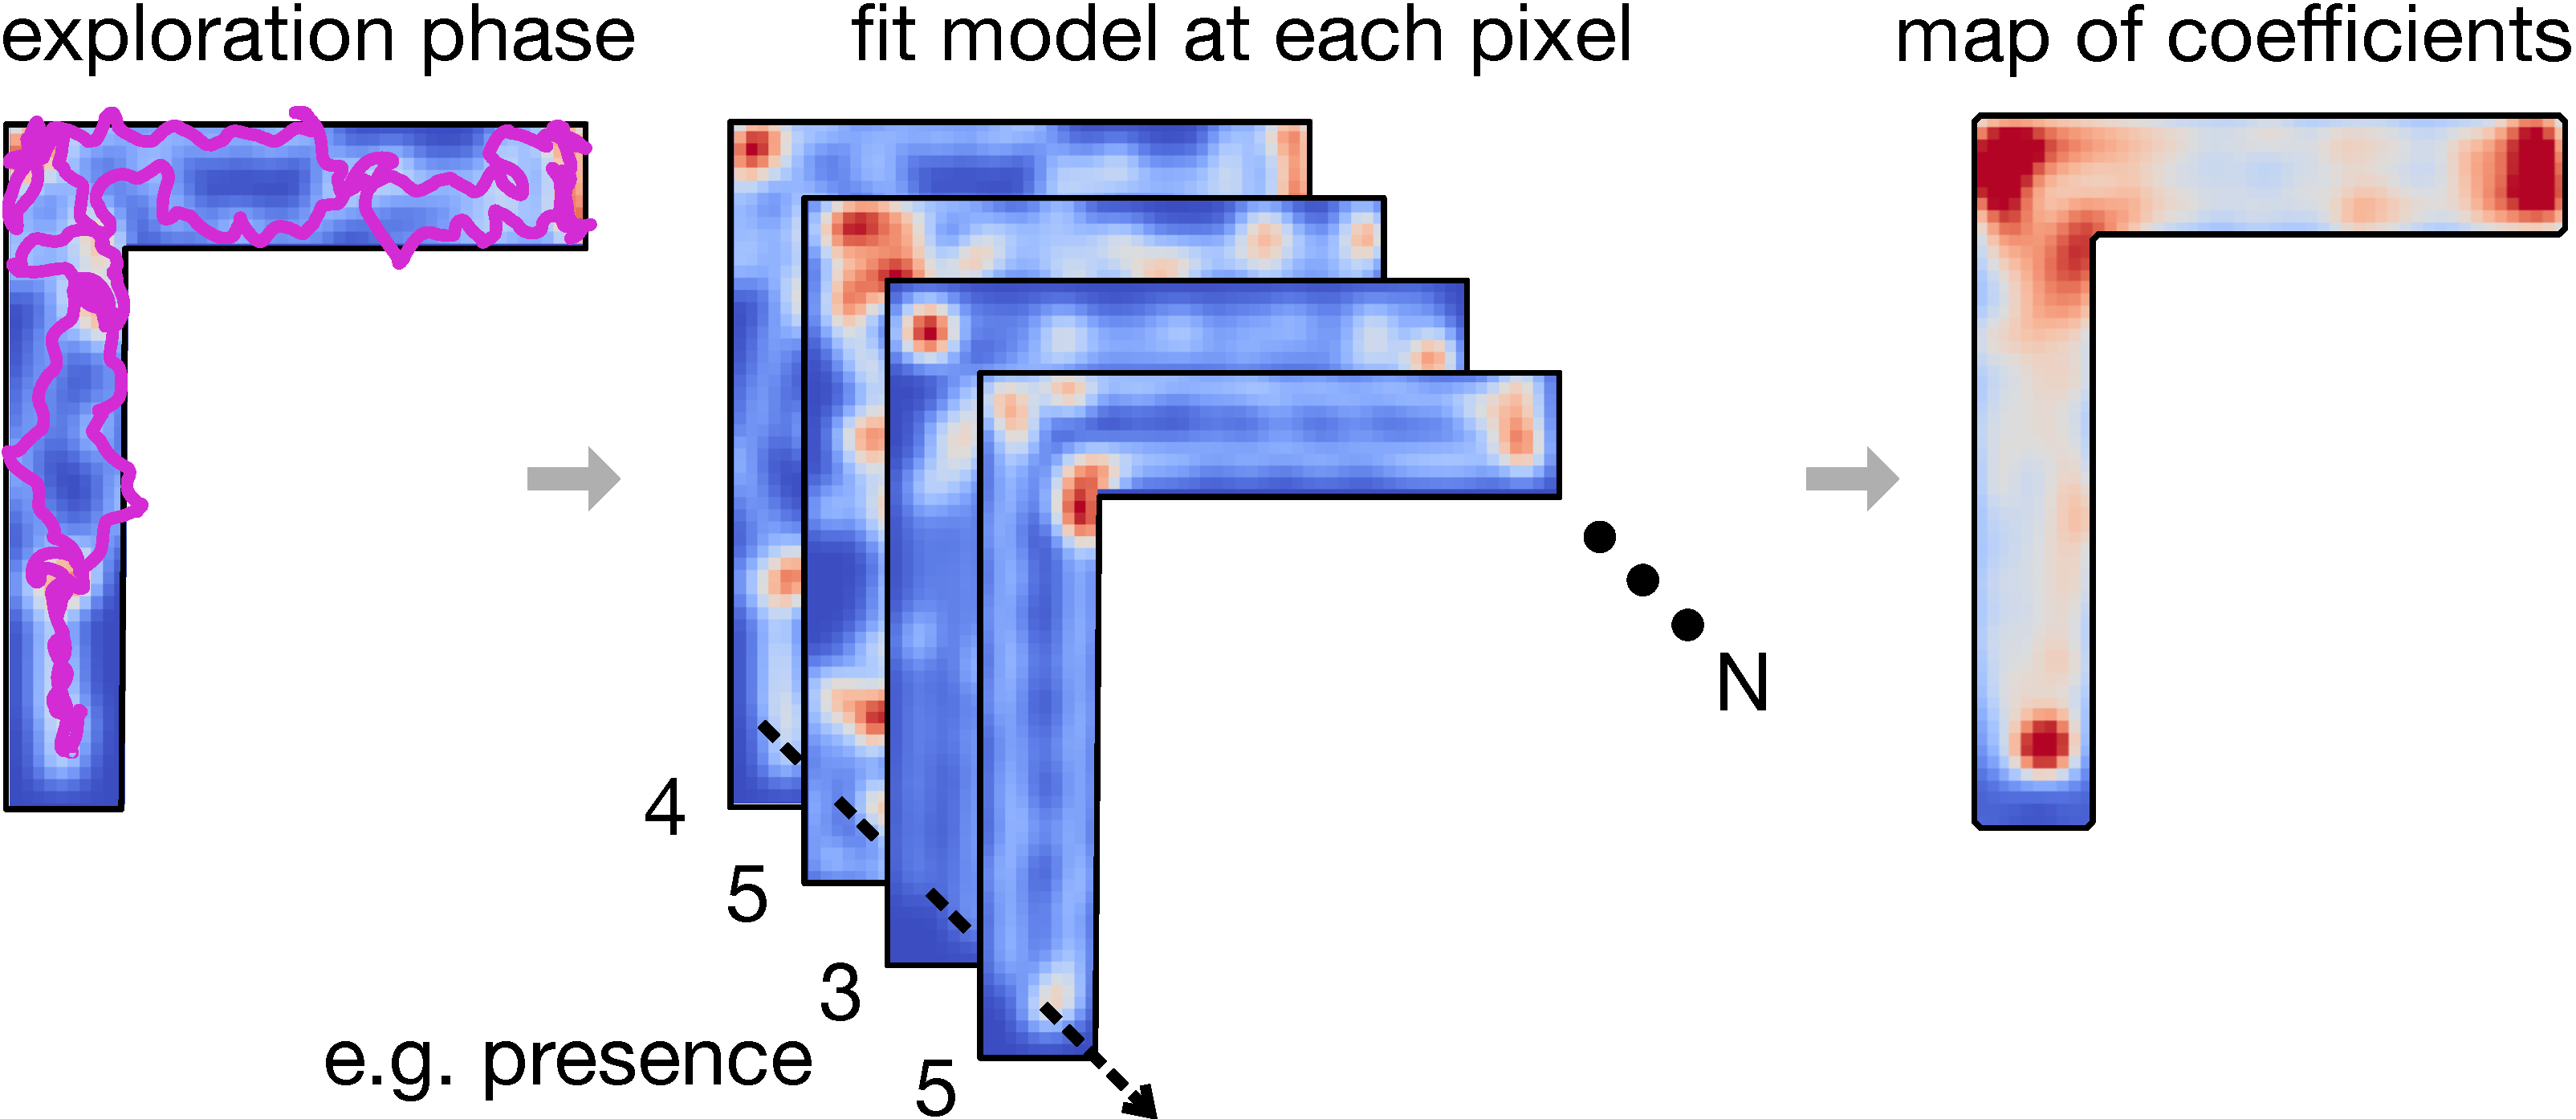
\includegraphics[width=\linewidth]{figures/methods.pdf}
  %\vspace{-15pt}
  \caption{Insert a caption below each figure. Do not alter the
    Caption style.  One-line captions should be centered; multi-line
    should be justified. }~\label{fig:methods}
\end{figure}